
Four points had to be clear before the development of the model started: what the system was
supposed to do, how its success would be measured, which limits it must obey, and what
resources it had. Setting these points out early ensured that the later assessment was fairer.
As an illustration, Chapter~\ref{ch:results} is able to show clearly that the system could not
comply with the clinical error limits for all seven antibiotics, because those limits had been
defined in advance. The broader impacts of the work, such as societal and environmental impact,
ethical concerns, standards, project planning, risks, and cost, are also discussed in this
chapter.

\section{Final Specifications and Requirements}
\label{sec:specs}

The requirements were based on the literature analysed in Chapter~\ref{ch:lit}~\cite{Kim2022,
Sakagianni2023}, the available data, and supervisor reviews after every stage. No clinician,
clinical microbiologist or laboratory technician was consulted. This represents an important
limitation, as the requirements were not verified directly with those who would use such a
system.

\subsection{Functional Requirements}

The system has an impact on clinicians, microbiologists, health services, researchers, and
patients. However, the requirements relate mainly to clinicians and patients, because they are
the ones who bear the cost of an incorrect prediction. Even a high average score may conceal a
severe case in which a resistant isolate has been reported as susceptible. Thus, the error
rates for every drug are recorded and the very major errors are measured
separately~\cite{Kim2022, Hu2024, who_amr_2019, Yu2025}. The ten requirements listed in
Table~\ref{tab:funcreq} were established prior to development. FR9 was the only one revised
later, for the reason given below.

{\small\setlength{\tabcolsep}{5pt}
\begin{longtable}{|l|>{\raggedright\arraybackslash}p{3.0cm}|>{\raggedright\arraybackslash}p{9.8cm}|}
\caption{Functional requirements of the proposed system.}
\label{tab:funcreq}\\
\hline
\textbf{ID} & \textbf{Requirement} & \textbf{What it means} \\
\hline
\endfirsthead
\hline
\textbf{ID} & \textbf{Requirement} & \textbf{What it means} \\
\hline
\endhead
\hline
\multicolumn{3}{r}{\footnotesize\textit{Continued on the next page}}\\
\endfoot
\hline
\endlastfoot
FR1 & Genomic input &
The system must accept whole genome information for \textit{Escherichia coli}. It must build
SNP features and gene presence or absence features automatically, without a bioinformatician
editing them by hand. \\
\hline
FR2 & More than one lens on the genome &
The system must describe each isolate's genome through more than one lens, so that
variant-level and gene-level information are both available to the model. \\
\hline
FR3 & Prediction for several drugs &
The system must predict resistant or susceptible for seven antibiotics covering five drug
classes. The penicillins are ampicillin (AMP) and amoxicillin with clavulanic acid (AMC); the
cephalosporins are cefotaxime (CTX) and ceftazidime (CAZ). Ciprofloxacin (CIP) is a
fluoroquinolone, gentamicin (GEN) an aminoglycoside, and trimethoprim with sulfamethoxazole
(SXT) a folate pathway inhibitor. \\
\hline
FR4 & Score instead of a plain label &
The system must return a score for each drug rather than a yes or no answer, so that the user
decides where the cut-off falls. \\
\hline
FR5 & Separate cut-off per drug &
The system must allow a different decision threshold for each antibiotic, because the cost of
a given error is not equal across drugs. \\
\hline
FR6 & Handling of missing labels &
The system must be trained with isolates tested against only some of the seven drugs, since
natural collections only test a small proportion of isolates for each drug. A boolean mask is
included with the label matrix, so
an untested drug is not read as a susceptible result nor is it allowed to contribute a
gradient. \\
\hline
FR7 & Interpretability output &
The system must produce interpretability output for every prediction. That output names the
genes which received the highest attention weights and the weight the gate placed on each
lens. \\
\hline
FR8 & Statistical reporting &
The system must produce bootstrap confidence intervals and significance tests against
competing models as part of its ordinary output. \\
\hline
FR9 & More than one kind of split &
The system must be evaluated under three splits: a random split, a phylogroup-stratified split
matching lineage composition across partitions, and a lineage holdout in which no sequence
type appears in more than one partition. The effect of relatedness on the reported score is
then measured at more than one level of detail. \\
\hline
FR10 & External validation &
The system must be evaluated on a different isolate collection that was used neither for
training nor for model selection. \\
\end{longtable}}

FR8, FR9 and FR10 were added from the beginning, since evaluation is core to this research. The
key question is not only whether resistance can be predicted, but also whether the model learns
resistance biology or population structure~\cite{Yu2025}. FR9 originally requested a random
split and a phylogeny-aware split. The initial phylogroup-stratified split resulted in balanced
broad lineages but no separation of close relatives. Thus, FR9 was amended to require a
sequence-type lineage holdout. This change is explained as Risk R1 in Section~\ref{sec:risk}.

\subsection{Non-Functional Requirements}

The performance targets were set prior to the final evaluation. They were fixed as minimum
acceptable levels and not as hoped-for results, to minimise the risk of adjusting the model
until it matched the test set. Table~\ref{tab:nonfuncreq} shows the non-functional requirements
that were identified and how each of them was verified.

{\small\setlength{\tabcolsep}{5pt}
\begin{longtable}{|l|>{\raggedright\arraybackslash}p{2.7cm}|>{\raggedright\arraybackslash}p{6.0cm}|>{\raggedright\arraybackslash}p{3.6cm}|}
\caption{Non-functional requirements and how each was verified.}
\label{tab:nonfuncreq}\\
\hline
\textbf{ID} & \textbf{Requirement} & \textbf{Target} & \textbf{How it was checked} \\
\hline
\endfirsthead
\hline
\textbf{ID} & \textbf{Requirement} & \textbf{Target} & \textbf{How it was checked} \\
\hline
\endhead
\hline
\multicolumn{4}{r}{\footnotesize\textit{Continued on the next page}}\\
\endfoot
\hline
\endlastfoot
NFR1 & Predictive quality &
Mean precision-recall AUC must reach at least 0.80 across the seven drugs on the random split.
Precision-recall AUC replaces accuracy because the classes are
imbalanced~\cite{saito2015, davis2006}. The target applies to the random split alone, since
that is the split carrying the baseline comparison; lineage-holdout results are reported
separately and are not measured against it. &
Measured on a held-out test set. \\
\hline
NFR2 & Statistical rigour &
Headline comparisons must carry a bootstrap confidence interval, and headline results must be
reported on all three splits. &
Bootstrap resampling, 1{,}000 rounds. \\
\hline
NFR3 & Reproducibility &
A fixed seed must reproduce output exactly, with every experiment setting under version control
and every training run logged. &
Reported numbers re-created from saved settings. \\
\hline
NFR4 & Training cost &
Full training must complete on one consumer GPU in hours rather than days. &
Fit times recorded for all experiments. \\
\hline
NFR5 & Inference speed &
Prediction for all seven drugs must take under one second per isolate once the genome is
assembled. &
Timed on the target workstation. \\
\hline
NFR6 & Memory &
The complete gene presence and absence matrix, before any gene filtering is applied, must fit
in the working memory of a single workstation. Its dimensions are the isolate and gene counts
given in Table~\ref{tab:constraints}. &
Peak memory monitored while the unfiltered matrix was built. \\
\hline
NFR7 & Interpretability &
Attention and gate weights must be available for every prediction and rankable by gene for each
drug. &
Per-drug gene ranking tables were produced. \\
\hline
NFR8 & Honest reporting of failure &
Clinical error limits that are not met must be reported as unmet, not hidden by selecting a
convenient threshold. &
Clinical error rates reported at a fixed threshold. \\
\hline
NFR9 & Maintainability &
Stages must be separable, so that changing one stage does not force the whole pipeline to be
re-run. &
Each stage writes its output before the next begins. \\
\hline
NFR10 & Improvement over the baseline &
Mean precision-recall AUC must exceed 0.803, the project's first classical baseline. That
baseline is an XGBoost model on 1{,}024 principal component features, built before the
gene-level baseline of Stage 2. NFR1 fixes an absolute floor; this requirement fixes a
relative one, against the project's own starting point. &
Compared drug by drug against the recorded baseline results. \\
\hline
NFR11 & Clinical error limits &
Very major and major error rates must both fall inside the CLSI limit for every drug at the
chosen operating point. &
Checked per drug and saved in the clinical metrics output. \\
\end{longtable}}

The mean precision-recall AUC of the final system was 0.849. This beat NFR1 by 0.049 and the
original baseline in NFR10 by 0.045. That baseline was not even: it ranged from 0.655 for
gentamicin to 0.948 for ciprofloxacin. The mean, however, masks significant variations between
the drugs. The improvement varied from 0.125 for trimethoprim-sulfamethoxazole to just 0.0005
for amoxicillin-clavulanate. Both models round to 0.748 for the latter. The majority of the
gain was also observed prior to the inclusion of the neural components. The classical model
improved from 0.803 to 0.830 when replacing principal components with gene-level features. The
best single classical learner eventually reached 0.840, leaving the final system only 0.009
ahead. This stronger baseline was not taken into account when defining NFR1 and NFR10.

\subsection{Constraints}

There were four conditions in the data and project setting that were fixed for the design.
These were not modelling choices; they were restrictions imposed on any prospective design.

{\small\setlength{\tabcolsep}{5pt}
\begin{longtable}{|>{\raggedright\arraybackslash}p{2.8cm}|>{\raggedright\arraybackslash}p{5.0cm}|>{\raggedright\arraybackslash}p{6.1cm}|}
\caption{Design constraints and their effect on the system.}
\label{tab:constraints}\\
\hline
\textbf{Constraint} & \textbf{Description} & \textbf{Effect on the design} \\
\hline
\endfirsthead
\hline
\textbf{Constraint} & \textbf{Description} & \textbf{Effect on the design} \\
\hline
\endhead
\hline
\multicolumn{3}{r}{\footnotesize\textit{Continued on the next page}}\\
\endfoot
\hline
\endlastfoot
Sample size & 6{,}962 labelled isolates in 8 phylogroups, a large number for genomic resistance
prediction and a small one for deep learning~\cite{goodfellow2016dl} &
Large neural models were ruled out. The design had to pair a small neural component with
classical learners rather than scale up. \\
\hline
Class imbalance & Some drugs, gentamicin above all, carry far fewer resistant than susceptible
isolates &
Accuracy carries no information here. Precision-recall AUC and MCC were used
instead~\cite{saito2015}, and confidence intervals became mandatory. \\
\hline
Number of features & 535{,}439 candidate SNP features and a pan-genome catalogue of 32{,}441
genes against only 6{,}962 isolates &
Heavy feature reduction was required before modelling, down to 5{,}000 genes, because every
extra free parameter is capacity to fit noise. \\
\hline
No laboratory access & The project is computational throughout, with no means of checking a
prediction by culture &
Every claim is a claim about data, not about biology confirmed at the bench. Interpretability
findings are hypotheses to be tested, not proven mechanisms. \\
\end{longtable}}

The greatest constraint is the absence of laboratory facilities. When the model gives high
importance to a gene, it only reflects that the model used that feature. It cannot demonstrate
that the gene is responsible for resistance. Laboratory experiments beyond the scope of this
research would be needed to confirm such a mechanism.

\subsection{Delivered System Specification}

These requirements led to TriLens-MoE-Stack. Three neural lenses model the genome in three
different ways and are then combined via a mixture-of-experts gate for each isolate and drug.
Their outputs are used with five classical base learners, followed by a separate logistic
regression meta-learner for each drug. Chapter~\ref{ch:method} details the complete
architecture and training process. All values reported here are found in the saved experiment
configurations.

The data are based on the Arcadia \textit{E. coli} collection~\cite{arcadia2024,
morin2024ecoli}. Table~\ref{tab:constraints} lists its size and the number of features in it,
and the rules of filtering are provided in Section~\ref{sec:data}. Each of the seven drugs,
AMP, CIP, AMC, SXT, GEN, CTX, and CAZ, is predicted in the three settings defined in
Section~\ref{subsec:splits}: a random split, a phylogroup-stratified split, and a sequence-type
lineage holdout. The external test is not a held-out test of this model. The two collections
have no features in common. Thus, only the classical stacking part was rebuilt on the Giessen
collection, with the four shared drugs and without the neural lenses.

\subsection{Compliance Against Requirements}

Figure~\ref{fig:requirements_status} summarises the outcome for all twenty-one requirements at
a glance, and the paragraphs below give the reasons.

\begin{figure}[H]
\centering
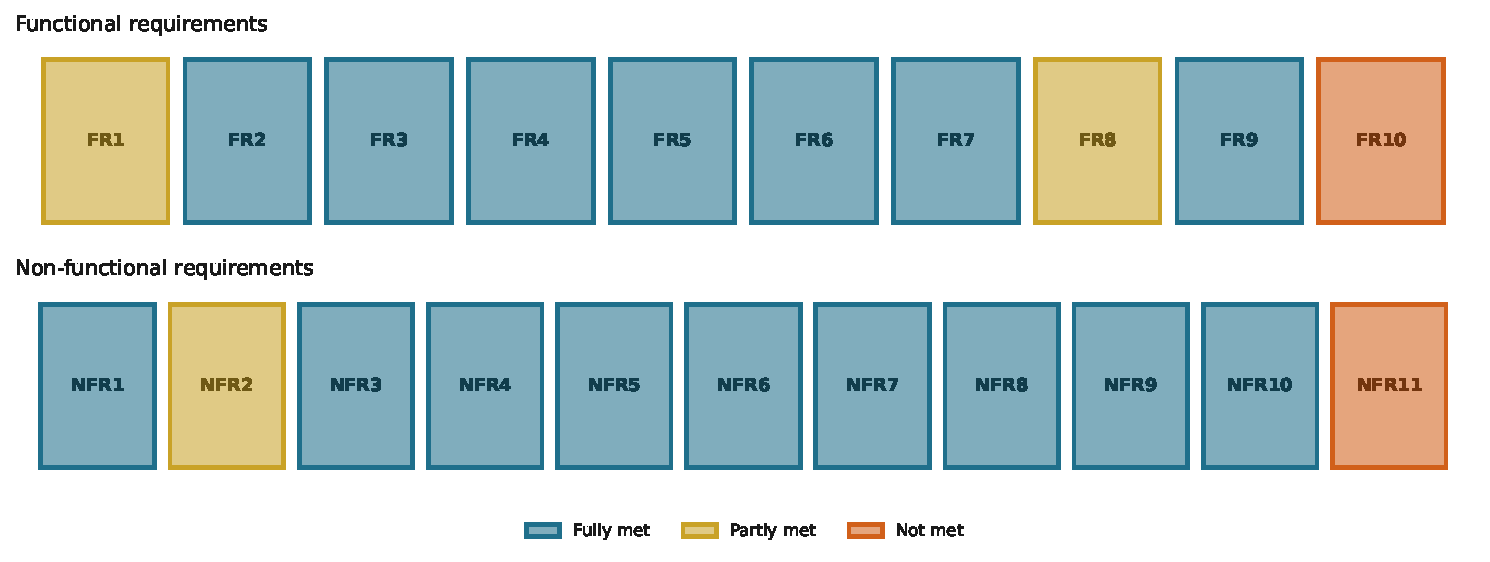
\includegraphics[width=\textwidth]{fig_requirements_status.pdf}
\caption{Compliance against every requirement fixed in advance.}
\label{fig:requirements_status}
\fignote{Of the ten functional requirements seven were fully met, two partly met and
one not met; of the eleven non-functional requirements nine were fully met, one
partly met and one not met. FR10 and NFR11 are the two that were not met.}
\end{figure}

Ten functional requirements were defined. Seven of them were fully met, two were only partly
met, and one was not met. FR1 was partially fulfilled, as features were generated from
existing variant calls in Arcadia, not directly from raw sequencing reads. FR8 was also
partially fulfilled, since baseline differences were evaluated using bootstrap intervals rather
than formal tests of significance. FR10 was not achieved, as the classical stack was retrained
on the Giessen collection rather than using a single fixed Arcadia-trained model.

Eleven non-functional requirements were defined. Nine of them were fully met, one was only
partly met, and one was not met. The mean score was 0.849, which is higher than the target of
0.80, so NFR1 was
met. Gentamicin (0.704) and amoxicillin-clavulanate (0.748), however, were still below 0.80
individually. NFR10 was met on average, and every drug scored at or above its own baseline,
though for amoxicillin-clavulanate the margin was only 0.0005. NFR2 was only partially
achieved, since confidence intervals were provided for the key comparisons but not for every
table in Chapter~\ref{ch:results}.

NFR11 was not met. The CLSI acceptance limits are 0.03 for major and very major errors.
Ciprofloxacin (0.015), gentamicin (0.023), and cefotaxime (0.026) fulfilled the major error
limit. However, no drug met the very major error limit, which ranged from 0.086 for
ciprofloxacin to 0.436 for gentamicin. Thus, no drug met both thresholds. Full results are
presented in Table~\ref{tab:clinical} in Chapter~\ref{ch:results}, with effects on responsible
use highlighted in Chapter~\ref{ch:conclusion}.

\section{Societal Impact}
\label{sec:societal}

A system that fails to catch resistance in every drug cannot be evaluated on its scores alone.
Its value is determined by what a clinician would do with it and by whom it would help.
Effective antibiotics are critical to many modern medical applications, such as surgery,
caesarean deliveries, chemotherapy, organ transplantation and care of premature
infants~\cite{who_amr_2019}. Antibiotic resistance reduces this protection, especially in
settings where few alternative drugs are available. There are few new classes of antibiotics,
so the existing ones must be used more carefully. Early prediction of resistance can help with
this, by making clinicians aware of the drugs that are unlikely to be effective.

Typically, culture-based susceptibility testing requires one or two days, since it involves
growing the organism and testing it against multiple drugs~\cite{Kim2022, Ren2022}. Treatment
can begin even before the result is available. A clinician can opt to use a drug that fails, or
resort to a broad-spectrum drug which is safer. The latter option can benefit the current
patient, yet it adds to the antibiotic pressure. The goal of good stewardship is to select the
narrowest effective drug for the shortest possible time~\cite{who_amr_2019}. An early
prediction can help with that decision while the laboratory result is still pending.

The situation is even more serious where laboratory testing is limited. In Bangladesh and other
South Asian countries, full susceptibility testing is mainly accessible in big cities, and
antibiotics can be purchased over the counter~\cite{who_amr_2019, Branda2024}. Treatment can be
initiated prior to the collection of a sample, and antibiotic courses can be discontinued when
the symptoms subside. These problems cannot be solved by a prediction system alone. Prescribing,
laboratory access, and clinical practice would also need to change to achieve better outcomes.
This work is intended to offer information; it is not a complete behavioural or health-system
solution.

There are practical benefits of a computational system. It does not require reagents, kits, or
cold storage, and a trained model can be replicated or retrained with local data. However,
sequencing is still required. Additionally, many resistant isolates are missed, including 0.436
for gentamicin and 0.394 for amoxicillin-clavulanate. So it should aid laboratory testing, not
replace it. At present, the system functions better as a regional resistance monitoring tool
than in making treatment decisions for individual patients.

Further constraining use of the system is the error pattern. Four of the drugs had major errors
below 0.04, but only three fell within the CLSI limit of 0.03. Very major errors were between
0.086 and 0.436, and were above the limit for every drug. Thus, the model can be useful for
identifying drugs that should be avoided until culture results are received. A drug should not
be prescribed only because the model predicts that it will be susceptible.

There is also an equity issue with the generalisation results. Performance was lower under the
sequence-type lineage holdout, when close relatives were excluded from training, and the extent
of the decrease was drug-dependent. This indicates that some of the predictive power of the
model comes from population structure instead of resistance biology~\cite{Yu2025}. Europe and
North America are also dominant in public genome collections~\cite{Yu2025}. Consequently,
models can perform poorly on underserved populations that already have limited access to
diagnostics. For this reason, all three data splits are reported and their differences are
regarded as an important result.

\section{Environmental Impact}
\label{sec:environment}

The argument presented above hinges on prescribing fewer and narrower spectrum antibiotics.
This would also be the most substantial environmental gain from this work, but it is by no
means the only quantity involved. Computation is a cost in itself, and it is only that side
which can be estimated from this project.

All experiments ran on one consumer GPU workstation. No cloud or cluster resources were required
and mixed precision was employed throughout. The longest full run was approximately 140 minutes
in duration. Across all experiments, the approximate energy consumption was 20--30 kWh. This is
just an estimated figure as no power meter was used. While low energy use was not a formal
goal, the final designs were both accurate and relatively cheap to run.

The potential for an environmental benefit is reduced antibiotic use. Antibiotic residues end
up in water and soil, where they continue to select for resistance~\cite{Liu2024}. This
pressure could be lowered with more targeted treatment. Some laboratory materials, such as
plates and media, may also be saved by computational prediction. Neither of these effects was
measured, however, and confirmatory culture is still necessary because of the current error
rates. The trained model is inexpensive to replicate, and will require retraining in the
future, as circulating lineages evolve.

\section{Ethical Issues}
\label{sec:ethics}

Counting energy and materials is easy, whereas it is more difficult to count the duties imposed
by a clinical system. They are not removed by writing correct code. This project was
guided by six duties: privacy, harm, equity, research integrity, benefit sharing, and dual use.

This is not a set of human genomes, but rather bacterial genomes. All data came from an open
community repository~\cite{morin2024ecoli, york2025amr}. No patient identifiers, clinical notes
or treatment records were involved. The pipeline only reads genome and sample identifiers,
phylogroups and antibiotic labels. No isolate was associated with an institution or person.

The main risk is over-reliance on the prediction. A very major error may result in a
non-functional drug, and none of the drugs passed the required limit. The system is also
described throughout as unvalidated for clinical use, and intended only as decision support alongside
laboratory testing, as mentioned in Section~\ref{sec:societal}.

The model is more accurate if there are related strains in the training set, and this is not
uniformly distributed across populations~\cite{Yu2025}. For this reason, the performance
difference between the three evaluation splits is made transparent.

Often, resistance prediction models appear good, but are not effective when careful testing is
conducted~\cite{Hu2024}. Three practices were used to avoid this. First, not only the direction
of each improvement is reported but also the size. This contains a negative finding: a more
complex neural meta-learner was worse than the simple one. The small margin mentioned in risk
R8 in Section~\ref{sec:risk} is also reported publicly. Second, a malfunction in the
resistance-gene keyword filter was discovered during the project, fixed, and the analysis
re-run. It is listed as R5 in Table~\ref{tab:risks}. Third, before the final comparisons, all
thresholds and protocols were set. Seeds, configuration files and run logs were saved, and thus
any reported number can be reproduced.

It is a more difficult question to ask who benefits than it is to ask who is harmed. The data
imbalance described in Section~\ref{sec:societal} indicates that the population with the
greatest impact from resistance is not the most well represented in this data set. This gap is
not due to a modelling decision in this project, but rather is due to the data available.
However, some measures were taken to ensure that it did not become worse. All libraries and
genomes used are open. The pipeline runs on a single consumer graphics card, and not on cluster
time. Errors are also reported per drug, so another group working on another local lineage can
see exactly what it would inherit.

The dual-use risk is low. Predicting resistance is not a means to produce or transfer
resistance. The algorithms and data are all publicly available, but the work also depends on
access to the organism and sequencing capacity.

\section{Standards}
\label{sec:standards}

Many of those responsibilities rely on being comprehended. If someone reading an error rate for
each drug cannot tell which errors matter, it helps no one, so this work borrowed its
vocabulary rather than inventing one. Although the system is not clinically validated, the
errors it identifies are characterised in terms already used by diagnostic practice. The
standards and codes of practice applied to the work are shown in Table~\ref{tab:standards}.

{\small\setlength{\tabcolsep}{5pt}
\begin{longtable}{|>{\raggedright\arraybackslash}p{3.3cm}|>{\raggedright\arraybackslash}p{3.2cm}|>{\raggedright\arraybackslash}p{7.4cm}|}
\caption{Standards and codes of practice applied to the work.}
\label{tab:standards}\\
\hline
\textbf{Standard or practice} & \textbf{Area} & \textbf{How we used it} \\
\hline
\endfirsthead
\hline
\textbf{Standard or practice} & \textbf{Area} & \textbf{How we used it} \\
\hline
\endhead
\hline
\multicolumn{3}{r}{\footnotesize\textit{Continued on the next page}}\\
\endfoot
\hline
\endlastfoot
CLSI susceptibility reporting & Clinical microbiology &
Errors are reported as per the standard definitions: very major error (VME), major error (ME)
and categorical agreement, following the clinical evaluation practice described for machine
learning based resistance prediction~\cite{Kim2022, Hu2024}. The result for each drug is
compared against the limits and reported. \\
\hline
Reproducible-research practice & Configuration, seeding and logging &
Hydra configuration files are versioned and kept separate from the code, and the seed is set to
42 for splitting, initialisation, folds and bootstrap. All training runs, including discarded
ones, are recorded externally, so the settings behind any reported number can be recovered
exactly. \\
\hline
Open source licensing & Software &
All libraries used by the pipeline are openly licensed, so the pipeline can be shared and
reused freely. \\
\hline
University academic integrity policy & Research conduct &
All sources cited, all negative results reported, no selection of favourable runs. \\
\end{longtable}}

CLSI reporting is especially critical since common machine learning metrics do not provide
direct indications of patient-safety risk. Accuracy, ROC-AUC, and F1 are commonly
reported~\cite{Hu2024}, whereas precision-recall AUC is more well-suited to imbalanced
classes~\cite{saito2015, davis2006}. But these measurements are primarily used to compare
models. Very major errors (VME), major errors (ME) and categorical agreement link the results
to clinical safety. The data were published for re-use~\cite{arcadia2024} and the software stack is open
source, meaning that the pipeline can be reimplemented and expanded.

These standards were followed voluntarily in this research. Much more would be needed for
clinical deployment. Programs that have an impact on diagnosis or treatment are typically
considered a medical device, and machine learning further introduces new challenges since
performance is dictated by the training data~\cite{Duggirala2025}. Before patient use, formal
clinical validation, documented claims and regulatory approval would be required. None of these
steps have been performed.

\section{Project Management Plan}
\label{sec:planning}

The practice of reproducible-research, as shown in Table~\ref{tab:standards}, was incorporated
in the schedule and not just tacked on at the end. The results of each stage of the project
were stored prior to the next stage. This saved on the re-running of unnecessary results, and
established a clear connection between each result reported and its origin file. It also helped
achieve the reproducibility goal in NFR3. Project stages, deliverables and outcomes are shown
in Table~\ref{tab:phases}.

{\small\setlength{\tabcolsep}{5pt}
\begin{longtable}{|l|>{\raggedright\arraybackslash}p{3.0cm}|>{\raggedright\arraybackslash}p{9.6cm}|}
\caption{Project stages, deliverables and outcomes.}
\label{tab:phases}\\
\hline
\textbf{Stage} & \textbf{Focus} & \textbf{Deliverable and outcome} \\
\hline
\endfirsthead
\hline
\textbf{Stage} & \textbf{Focus} & \textbf{Deliverable and outcome} \\
\hline
\endhead
\hline
\multicolumn{3}{r}{\footnotesize\textit{Continued on the next page}}\\
\endfoot
\hline
\endlastfoot
1 & Data collection and preparation &
Genomes assembled, variants called, susceptibility labels extracted for seven drugs, and
training, validation and test splits defined and frozen. \\
\hline
1.5 & Feature reduction &
Chi-squared pre-filtering and XGBoost importance ranking to trim the feature space to
5{,}000 genes, with the number of genes retained at each step recorded for auditing. \\
\hline
2 & Classical baseline &
Gene-aggregated gradient boosting achieved approximately 0.830 mean precision-recall AUC,
establishing the baseline any proposed system had to exceed. \\
\hline
3 & Neural modules &
The mixture-of-experts and attention-based gene models were constructed. The result was
negative: no neural model alone performed better than the classical baseline. \\
\hline
4 & Stacking &
Several stacking designs were created, with classical and neural base learners communicating
via a meta-learner. It was found that interaction, not any one model, was the direction to
take. \\
\hline
5 & Final model and ablation &
The architecture was completed and a step-wise ablation was carried out to dissect the
contributions of fusion, the meta-learner and the decision threshold. \\
\hline
6 & Validation studies &
Locality testing, interpretability analysis, phylogroup-stratified evaluation and transfer to
an external collection generated the generalisation results. \\
\hline
7 & Statistical analysis &
Bootstrap confidence intervals, prevalence-matched resampling, threshold-tuning checks and
clinical error rates were calculated. \\
\hline
8 & Documentation &
Research report, figures, defence materials and the journal version of the work were prepared. \\
\end{longtable}}

The component stages of the model used in the ablation study in Chapter~\ref{ch:results} are
different from the stage numbers above, which are project phases.

Two consumer graphics cards were used in the work. An NVIDIA RTX 4080 SUPER was the main
device, and an RTX 4070 Ti was used for development, so one hardware failure could not stop the
project. The software was an open-source standard Python stack. The neural lenses and the gate
were implemented with the help of PyTorch and Lightning. XGBoost, LightGBM, and scikit-learn
were used for the classical base learners and the
meta-learner~\cite{chen2016xgboost, ke2017lightgbm, breiman2001rf}, and SHAP was used for
attribution. All the experiment configurations and training runs were recorded by Hydra and
Weights and Biases. Precise package versions are stored in the project environment file instead
of in this list.

There was no dedicated budget and the timeline relied on the time and computing capabilities of
a single workstation, as Section~\ref{sec:economic} outlines. The supervisor assessed the
progress following each stage and these assessments informed the subsequent stage. One review
switched the principal components for gene-level features, which resulted in a better baseline
of 0.830, while also being more interpretable. Another review decided to reject a neural
meta-learner because it gave worse results than logistic regression. All stages yielded a
usable product, which meant that if any later stages had not been included, the project could
have still been finished.

\section{Risk Management}
\label{sec:risk}

The main risks were established at the beginning of the project and re-evaluated at the end of
each project stage. All the risks in Table~\ref{tab:risks} have happened or were so severe as
to necessitate a clear control.

{\small\setlength{\tabcolsep}{5pt}
\begin{longtable}{|l|>{\raggedright\arraybackslash}p{4.3cm}|>{\raggedright\arraybackslash}p{1.5cm}|>{\raggedright\arraybackslash}p{1.4cm}|>{\raggedright\arraybackslash}p{5.0cm}|}
\caption{Project risk register with severity, occurrence and mitigation.}
\label{tab:risks}\\
\hline
\textbf{ID} & \textbf{Risk} & \textbf{Severity} & \textbf{Occurred} & \textbf{What we did} \\
\hline
\endfirsthead
\hline
\textbf{ID} & \textbf{Risk} & \textbf{Severity} & \textbf{Occurred} & \textbf{What we did} \\
\hline
\endhead
\hline
\multicolumn{5}{r}{\footnotesize\textit{Continued on the next page}}\\
\endfoot
\hline
\endlastfoot
R1 & Results are too good because related isolates appear in both the training and the test
set &
High & Yes &
Constructed a phylogroup-stratified split first, which failed to answer the question, followed
by a real sequence-type lineage holdout~\cite{Yu2025}. Rather than quietly patching the defect,
we report the correction as one of the principal findings. \\
\hline
R2 & Overfitting on a small and imbalanced dataset & High & Partly &
Early stopping with patience 8, regularised base learners, out-of-fold meta-learner inputs and
bootstrap confidence intervals on every score. \\
\hline
R3 & Results are valid only for the collection the model was trained on & High & Partly &
Rebuilt the classical stack independently on a second collection and measured the performance
retained by the method. \\
\hline
R4 & Insufficient resistant isolates for some drugs, making estimates unstable &
Medium & Yes &
Instead of accuracy, reported precision-recall AUC and MCC with confidence intervals, so that
the weaker drugs show clearly that they are less certain. \\
\hline
R5 & Interpretability analysis errors leading to incorrect biological claims & Medium & Yes &
A loose substring match in the resistance-gene keyword filter was reading an unrelated protein
domain as a resistance gene. Found in the Stage 6 interpretability analysis, analysis re-run,
false positive removed and true positive retained. \\
\hline
R6 & Annotation sources using different naming schemes & Medium & Yes &
One annotation source was not at all consistent with the gene identifiers. Only the source that
matched was analysed, and such restriction was mentioned. \\
\hline
R7 & Losing work due to hardware or run failure & Medium & No &
Outputs from every stage were saved, checkpointing was used for training, all runs were logged
externally, and there was a second card available. \\
\hline
R8 & The proposed system fails to separate, in any meaningful sense, from the strongest single
learner available to it & Medium & Yes &
Moved the claimed contribution towards interpretability, evaluation design and external
validation, and reported the size of the improvement alongside its direction. \\
\hline
R9 & Scope growing beyond the time available & Medium & No &
The staged plan gave each stage a usable deliverable, so the project would have remained
defensible if it had been reduced to the earlier stages. \\
\hline
R10 & Losing reproducibility through undocumented experiments & Medium & No &
Fixed seed of 42, versioned Hydra configuration files and external run logging from the first
stage onwards. \\
\end{longtable}}

There were five risks that took place completely and the other two partially. The most
significant ones were R1 and R8, as they altered the primary meaning of the research.

R1 is the risk that is most often missed in this field. There are large numbers of
near-identical isolates in a genomic collection. A random split can result in members of the
same group being on both sides, and the model may just be identifying a familiar strain. The
initial response was the phylogroup-stratified split. It ensured that the eight broad lineage
groups were balanced between the partitions, but it did not separate close relatives, as each
phylogroup was still represented on both sides. It thus assessed the impact of the
stratification variable, not generalisation to an unseen lineage. Its performance even improved
slightly under it, from 0.849 to 0.853. This was first read as robustness, before it became
apparent what the split could not test. It was replaced by the sequence-type lineage holdout,
which assigned whole sequence types to one partition only. Average precision-recall AUC then
dropped from 0.849 to 0.634, or to 0.723 after adjusting for the prevalence shift that such a
holdout introduces. Section~\ref{subsec:prevmatch} presents the per-drug figures. R1 was not
simply reduced. The correction changed the main conclusions of this research.

R8 also occurred fully. The final system is at the top of the baseline ladder in
Chapter~\ref{ch:results}. But its margin of superiority over the best single classical learner
is 0.009, which is less than the bootstrap interval for either score. Then, under the lineage
holdout in Section~\ref{sec:statanalysis}, the margin is reduced to 0.004: 0.630 for that
learner versus 0.634 for the full model. The claimed contribution was thus altered. This research
is not based on this model's ranking in the baseline, rather it is based on separating
biological mechanism from population structure for each antibiotic.

\section{Economic Analysis}
\label{sec:economic}

The direct cost of the project was extremely small. The software was open source, the genomes
were publicly available and the work was done with existing computers, not rented or bought
machines.

The primary cost was human labour. The work could be repeated by a small research group with
the requisite programming skills and with an appropriate workstation. Sequencing is still
costly, so the system is most viable in situations where genome information is already being
generated, such as outbreak monitoring. It is not a cheap alternative to culture-based testing.

A reliable cost--benefit value cannot be calculated from this study. Benefits may include
improved treatment and reduced sickness, reduced costs of narrow-spectrum drugs and extended
useful life of existing antibiotics~\cite{who_amr_2019}. If the forecast is incorrect, it can
lead to greater sickness or hospitalisation. The actual cost will vary based on the medication,
local resistance and the use of the outcome. A single monetary estimate would be misleading as
these factors were not measured.

The per-drug results still give a picture of the relative strengths of the system. The very
major error rate was lowest for ciprofloxacin (0.086). The weakest were gentamicin (0.436) and
amoxicillin-clavulanate (0.394). Since no drug met the CLSI limits, these figures only compare
the drugs; they do not show clinical readiness. Any subsequent application would have to be
looked at individually for each drug.
